
%----------------------------------------------%
% {{{
%----------------------------------------------%

\documentclass[12pt, a4paper, titlepage]{report}


%----------------------------------------------%
% Packages
%----------------------------------------------%


\usepackage{graphicx}   % Images
\usepackage{enumitem}   % Pretty lists
\usepackage{listings}   % Code listings
\usepackage{hyperref}   % Links

\usepackage[backend=biber]{biblatex}   % Bibliography
\bibliography{../rc/sources/AITools}   % Remember: no .bib
\bibliography{../rc/sources/manual}
\bibliography{../rc/sources/Maturawork2023}

%----------------------------------------------%
% Metadata
%----------------------------------------------%

\title{RtoV - Deep Learning with Generated Data for Raster Vectorization}
\author{Lars Hoesli}
\date{December 2023}


%----------------------------------------------%
% Macros, commands and definitions
%----------------------------------------------%

% Make title, author and date referable
\makeatletter\let\inserttitle\@title\makeatother
\makeatletter\let\insertauthor\@author\makeatother
\makeatletter\let\insertdate\@date\makeatother


%----------------------------------------------%
% }}}
%----------------------------------------------%



\begin{document}


%----------------------------------------------%
% Title page {{{
%----------------------------------------------%

\begin{titlepage}
    \centering

	 % Title
    \Huge{\textbf{\inserttitle}}
    \par
    \Large{Matura Work by \insertauthor}
    \vspace{1cm}\par
    \large{\insertdate}
    \vspace{2cm}

    % Title picture
    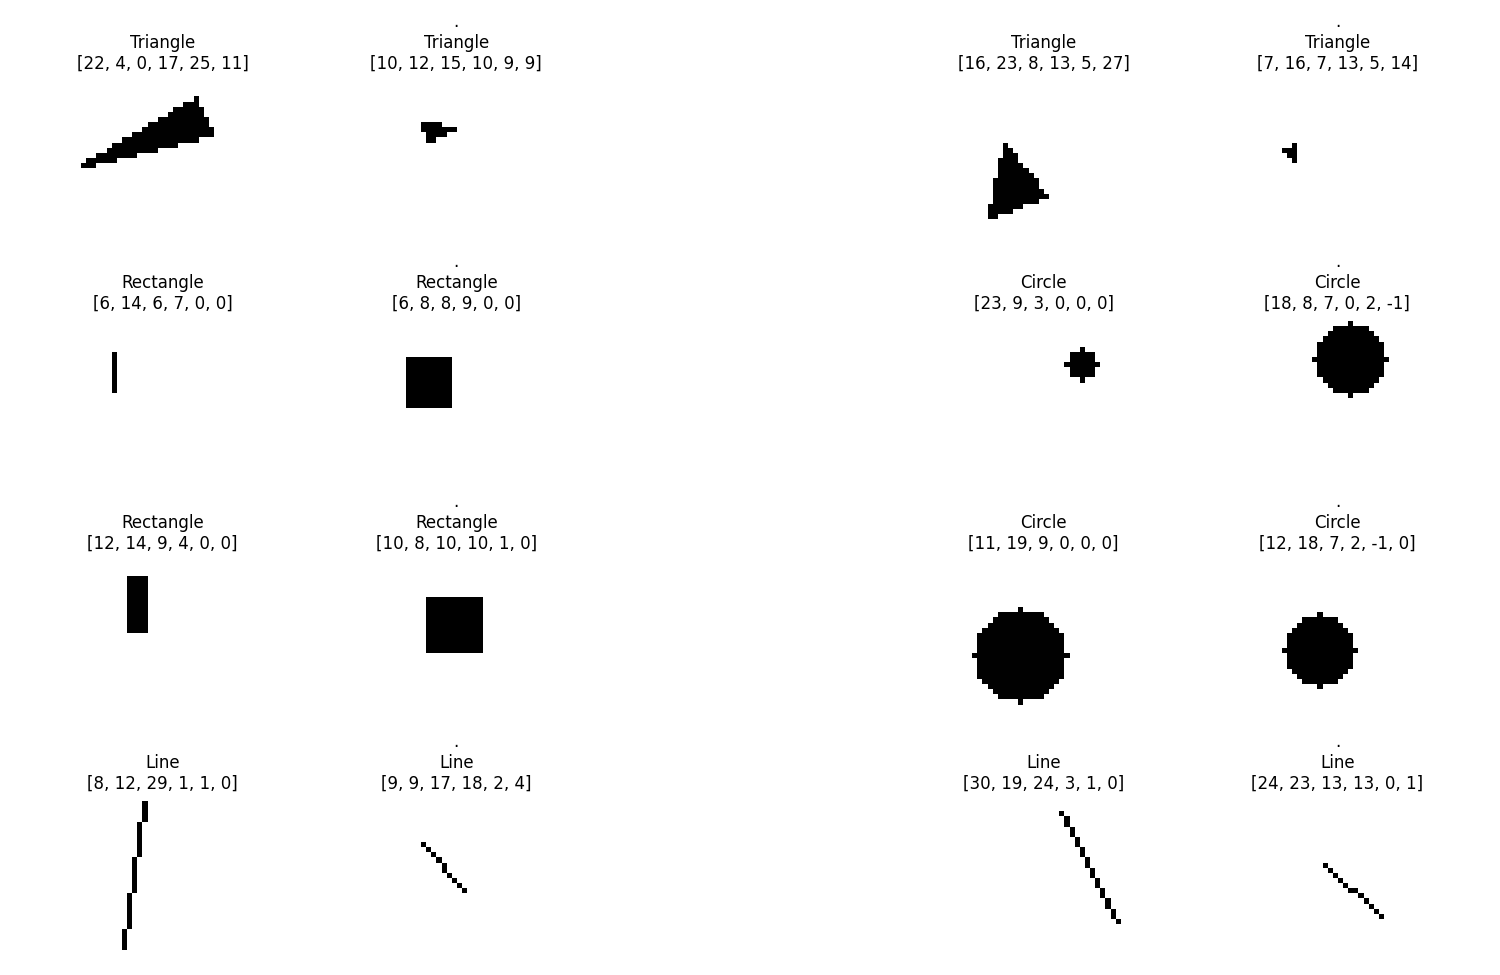
\includegraphics[width=1.0\textwidth]{../rc/images/all_shapes_approx_visual1.png}
    \vfill
    % Abstract
    \begin{abstract}
       The conversion from raster images to vector representations remains a challenging task to this day and is actively researched. Due to the inherent difficulties that algorithmic approaches face, such as finding shapes in noisy or blurred images with varying lighting conditions, much research is done using machine learning, where the most apparent problem is the acquisition of appropriate training data. Therefore, it can be beneficial if pairs of raster images and their corresponding vector representations could be automatically generated.

		 This paper examines this particular approach: Training a machine learning model on generated data pairs. A demonstration is done in a limited scope, where a deep learning model is trained on data that is generated on-the-fly in order to perform the conversion into a vector representation from raster images containing clearly visible shapes. The model used in the demonstration is a simple multi-task learning model with a Convolutional Neural Network as a frontend.

       \vspace{1cm}
       The code for the demonstration can be found online under \href{https://github.com/lrshsl/RtoV}{github.com/lrshsl/RtoV}
    \end{abstract}

\end{titlepage}

%----------------------------------------------%
% }}}
%----------------------------------------------%

%----------------------------------------------%
% Table of contents {{{
%----------------------------------------------%

\tableofcontents

%----------------------------------------------%
% }}}
%----------------------------------------------%



%----------------------------------------------%
% Introduction {{{
%----------------------------------------------%

\chapter{Introduction}

Images have become an important part of everyday live, most of which are stored digitally, which is making the search for effective storage of images an essential, well researched aspect of computer science.
Many different formats and compression have emerged, the most influential of which can be categorized into two main categories - vector and raster formats.

\section{Vector and Raster Graphics}

Vector and raster graphics are two fundamentally different approaches on how to represent the content of an image. Both have advantages in representing a certain kind of image, and are less appropriate in other situations. While raster images store the color values of small parts of a given picture - often called pixels - to approximate what the image looks like, vector formats rather store a specification for what shapes can be seen, similar to how humans receive images.

Both methods have pros and cons, and are more appropriate for certain situations than others. But vector formats have many advantages for storing images that are easily describable in shapes, especially shapes made up of one-colored areas or easily describable gradients. In such cases, vector graphics can represent those shapes more precise, with infinite resolution, while being less storage intensive at the same time. Raster formats in turn are better suited for images without easily distinguishable shapes, such as portraits or landcape images.

While format conversions among raster or vector formats and from vector to raster graphics can be done with a multitude of programs, the conversion from a raster image to a vector representation proves to bee more challenging, especially because the shapes and their features seen in the input image have to be recognized, which is not a easily solvable problem. Many factors can make it much more difficult, such as contrasts in different strengths, noise, and gradients that make it impossible to work with fixed thresholds to detect the contoures of shapes. With different manipulations, that one can apply to a given image, edge detection is made possible. That does not solve the problem though, since the composition of those edges still is difficult to do algorithmically.
With deep learning those problems can somewhat be overcome, since the model itself can recognize the shapes, in a similar manner as humans do. Deep learning models have their own difficulties, of which accumulating training data is a big limitation.

Therefore a way to convert raster images into a vector format is beneficial, and is not yet a solved problem. This is why I have chosen to do my matura thesis on the topic of raster to vector conversion.


\pagebreak

\section{}
\subsection{Activation Functions}
\subsection{Loss Functions}

\section{Architectures of Neural Networks}

Deep neural networks can be structured in different ways, leading to different kinds of traits that are beneficial in certain situations over others. For raster to vector conversion the following architectures are especially interesting.

\subsection{Convolutional Neural Networks}

A Convolutional Neural Network (CNN) is a type of neural network that uses a convolutional layer to extract features from an input image. It is useful to reduce the information of the single pixels to a sequence of single features, that fully connected layers then can learn to connect. In order to extract the relevant features, it uses different \emph{kernels}, which are moved through the images using a certain \emph{stride} value, and applied to the pixel values. The \emph{kernel} and \emph{stride} values can be used to reduce the information for the following layers directly. Alternatively after each convolution, a certain function can be applied, which reduces the features that need to be processed. A common architecture consists of repeating convolution and pooling layers, and finally fully connected neuronal layers that can process the information logically as it is seen in \ref{fig:cnn_architecture}.

\begin{figure}
	\centering
	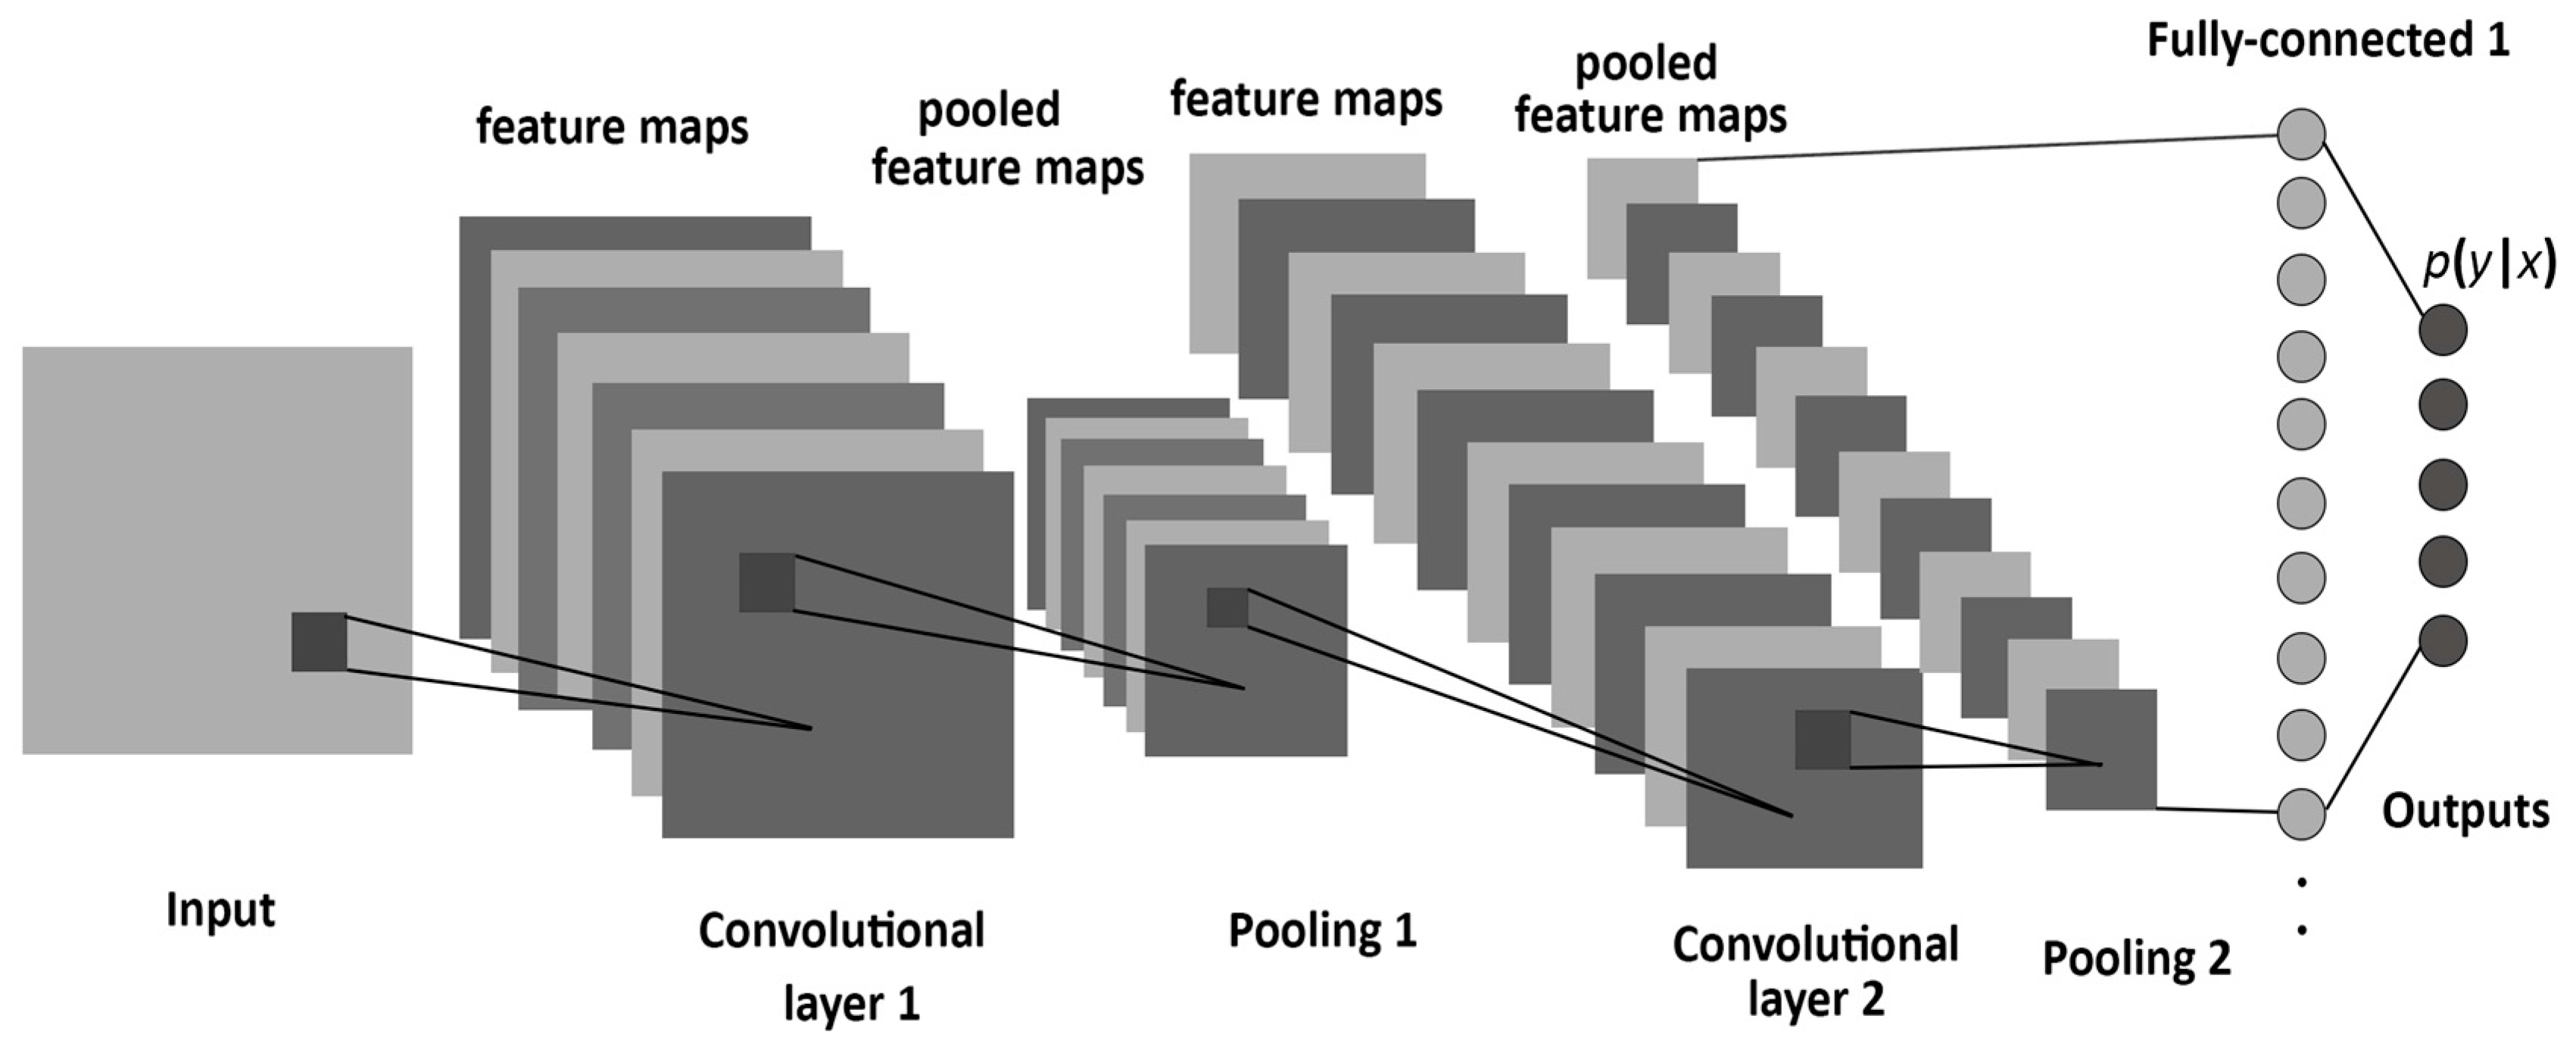
\includegraphics[width=1.0\textwidth]{../rc/images/cnn_architecture.png}
   \caption{Typical Convolutional Neural Network architecture \cite{img_cnn_architecture}}
	\label{fig:cnn_architecture}
\end{figure}


Convolutional Neural Networks have the advantage of being able to automatically identify relevant features in images. As such, they are used for computer vision, object detection as well as classification tasks. In the demonstration for this work, the CNN architecture is used to classify the image and extract the relevant features.


\subsection{Recurrent Neural Networks}

Recurrent Neural Networks (RNNs) well suited to handle sequential data by remembering information about previous inputs. This kind of memory mechanism is achieved by having loops within the neural network, allowing Recurrent Neural Networks to retain information and consider past in- and outputs when processing current ones. This makes them ideal for tasks like time series prediction, natural language processing, speech recognition, and more.

\begin{figure}
	\centering
	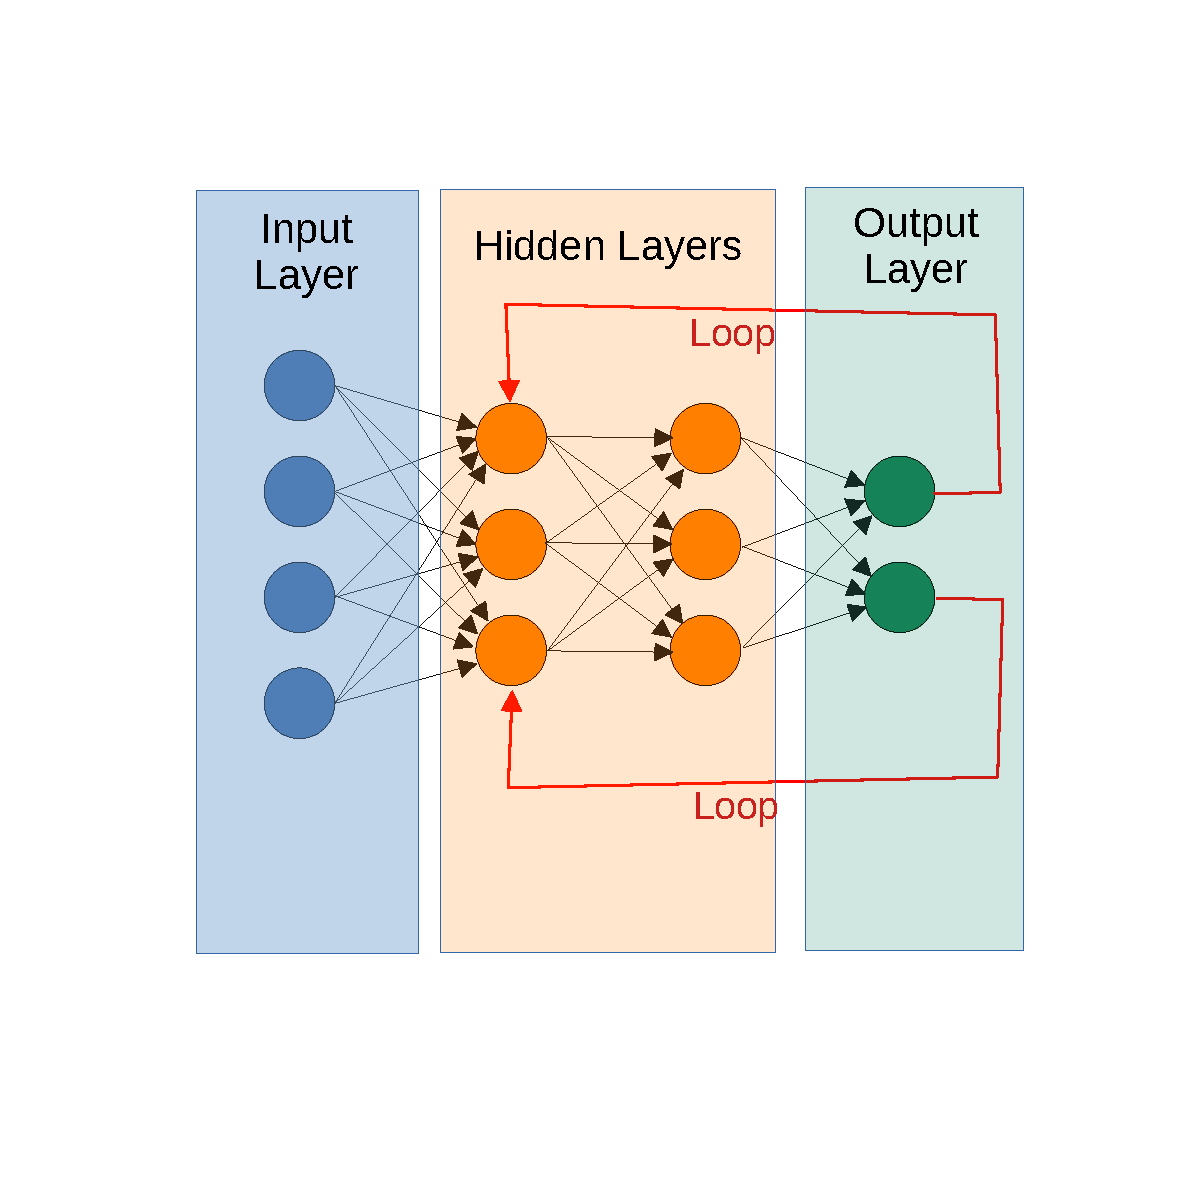
\includegraphics[width=1.0\textwidth]{../rc/images/rnn_architecture.pdf}
   \caption{Example Recurrent Neural Network architecture \cite{img_rnn_architecture}}
	\label{fig:rnn_architecture}
\end{figure}

However, traditional RNNs can face issues like the vanishing or exploding gradient problem, hindering their ability to learn long-range dependencies effectively.
To address those issues, improvements like Long Short-Term Memory (LSTM) and Gated Recurrent Unit (GRU) have been developed. These architectures use gating mechanisms that control the flow of information, enabling better long-term memory and gradient flow.

RNNs and their enhanced versions like LSTM and GRU have proven valuable in various applications that involve sequential data, allowing machines to comprehend and generate sequences more effectively than standard feedforward networks. In the case of raster vectorization this architecture could allow a neural network to remember which shape has previously been processed.

\subsection{Reinforcement Learning}

In Reinforcement Learning (RL), a neural network (agent) learns to make decisions by interacting with a given environment. The agent takes actions in the environment, and based on those actions, it receives feedback in the form of rewards or punishments. The goal of the agent is to learn how to maximize the reward.

The suggested use of RL for vectorization in this paper is inspired by the work "Marvel - Raster Manga Vectorization via Primitive-wise Deep Reinforcement Learning"  (\cite{su_marvel_2023}).

The agent learns by trial and error, exploring different actions and observing the consequences in terms of rewards. The goal is to discover an optimal policy that leads to the maximum cumulative reward over time. Reinforcement learning has been successfully applied to various domains, including game playing (e.g., AlphaGo), robotics, finance, and more. They have already proven valuable in raster to vector conversion \cite{su_marvel_2023}.

\begin{description}
   \item[Environment]: In the case of the raster to vector conversion, the environment is the raster image that is being converted.

   \item[State]: The state is a copy of the original image, which is modified by the agent each time a new shape is predicted.

   \item[Action]: The delection of the shape that was predicted follows as a action, that modifies the state.

   \item[Reward]: The reward is calculated by comparing the original image with the state. To do this comparison, both images would have to be converted into a raster presentation, so that the pixel values can be compared.
\end{description}

\section{Existing Approaches}

Raster to vector conversion is a well researched field, and there are many different approaches on how to do it. Apart from algorithm based strategies, machine learning and particularly neural networks are promising and in active development \cite{dziuba_image_2023}.

\subsection{Algorithmic Approaches}

\begin{enumerate}[label=\Roman*]
   \item \textbf{Edge Detection Techniques} Traditional algorithms often rely on edge detection methods to identify boundaries in raster images. These can be used to identify the shapes in the image, which can then be used to generate its vector representation.

   \item \textbf{Hough Transform} The Hough Transform is utilized to detect lines in raster images, serving as a foundation for vectorization. This approach is effective in representing straight lines but may face challenges with curves.

   \item \textbf{Skeletonization} Skeletonization algorithms aim to reduce shapes in raster images to their core structures, facilitating the extraction of vector representations.
\end{enumerate}

\subsection{Deep Learning Approaches}

\begin{enumerate}[label=\Roman*]
   \item \textbf{Convolutional Neural Networks (CNNs)} CNNs have been employed for raster-to-vector conversion by learning hierarchical features. They excel in capturing spatial relationships and are effective in handling complex patterns.

   \item \textbf{Autoencoders} Autoencoders, especially variational autoencoders (VAEs), have shown promise in capturing latent representations of raster images, which can be used for vectorization.

   \item \textbf{Generative Adversarial Networks (GANs)} GANs, known for generating realistic images, can be adapted to generate vector representations by training on paired raster-vector data.

   \item \textbf{Recurrent Neural Networks (RNNs)} RNNs, with their sequential learning capability, are suitable for tasks involving sequential data. They can be applied to capture patterns in raster images that than can be used for vectorization.

   \item \textbf{Attention Mechanisms} Models incorporating attention mechanisms, such as Transformer architectures, can focus on relevant parts of raster images during the vectorization process, improving accuracy.
\end{enumerate}

These approaches represent a spectrum of techniques, each with its strengths and limitations. Hybrid models that combine algorithmic and deep learning components have also emerged, aiming to leverage the benefits of both paradigms. As one of those, MarVel

%----------------------------------------------%
% }}}
%----------------------------------------------%


%----------------------------------------------%
% Goal and Hypothesis {{{
%----------------------------------------------%

\chapter{Goal and Hypothesis}

To train a machine learning model to vectorization of raster images, a substantial amount of data is needed. Ideal data would be pairs of raster and vector representations of the same image, which are difficult to obtain normally. Since the conversion of vector images to raster formats is far less difficult, it could be a valid approach to generate random vector images and them convert them into a raster format, to get those raster-vector pairs on which the model can be trained.


This work examines this approach in regard to the following questions:

\begin{enumerate}[label=\Roman*]
   \item Is it feasible to approach raster to vector graphics conversion with a neural network that is trained on randomly generated data?
   \item What strategies or measures have to be taken in order to make this feasible?
   \item What performance can be achieved, and what are the limitations and pitfalls of this approach?
\end{enumerate}


Furthermore, very specific questions are being asked:

\begin{enumerate}[label=\Roman*]
   \item How should the data be generated? In large chunks and stored on disk? Batches that are stored in memory?
   \item How should the model be trained?
\end{enumerate}

%----------------------------------------------%
% }}}
%----------------------------------------------%


%----------------------------------------------%
% Method {{{
%----------------------------------------------%

\chapter{Method}

\section{Overview}

The training and evaluation data for the model consists of 100x100 pixel images with 3 color channels, with exactly one shape on each image. The shape is being written on all color channels that are within the shape, and thus appears black on a white canvas when plotted. Which shapes is generated, as well as what the size and position of the shapes are, are randomized and differ on each call.

The training occurs in several steps:
\begin{enumerate}
   \item Generation of the training data
   \item Training of the model
   \item Evaluation of the model
\end{enumerate}


\subsection{Shape Generator}

A function has been written for each shape that returns a numpy array that describe the shape in as few bytes as possible. Since the number of datapoints differs from each shape, the array is padded with zeros to match the maximum number of datapoints. This padding is not being used for determining the performance of the model.

Here is a breakdown of the different shapes and their data representation:
\begin{itemize}
   \item Line: A line is defined through two points, width and color: [x1, y1, x2, y2, width, <color>]. Zeros are added for padding. Width and color are not used by the model in the demonstration.
   \item Circle: Center, radius and color: [x, y, r, <color>].
   \item Rectangle: One corner, width, height and color: [x1, y1, w, h, <color>].
   \item Triangle: Three corner points and color: [x1, y1, x2, y2, x3, y3, <color>].
\end{itemize}

When fully implemented, the color could take up 4 bytes, for red, green blue and alpha values. In the unmodified demonstration, the color is not being used, since the color that is being written on the image is always black.

The function in the current configuration returns a one dimenstional numpy array with a length of 6, which is the the number of datapoints used for a triangle (without color).


The corner points, width and height values that are generated are restricted in such a way, that the shape is always within the image. The possibility, that two different shapes can lead to the same pixels being colored, is not being taken into account though. Is thus is possible, that e. g. a triangle with its corners forming a line looks the same to the model.


The representation that is obtained after the previous step, then is written to a numpy array with the shape \lstinline{(100, 100, 3)} or in graphical terms a white canvas. For the conversion from this specific representation to a raster image, a function has been developed (the \lstinline{draw_on_image} function in \lstinline{data/draw_shape_on_image.py}) that performs this conversion with the help of the OpenCV2 library.

\subsection{Training}
\subsection{Evaluation}

For the evaluation of the model, its output, which is a numpy array containing the shape prediction and one which contains a specification in the same representation as the ground truth, is being compared to the original shape. This is done using the following loss functions: Sparse Categorical Crossentropy for the shape prediction and Mean Squared Error for the prediction of the other datapoints.


\section{Language Choice}  % {{{

Deep learning is a very resource intense task, and since the work was limited in time and resource usage, the language choice was taken in regards mainly to the expected development time and runtime performance of the language and their frameworks. And since the computational intensive parts are done within the deep learning library that is going to be used, the availability of performant and established machine learning libraries was a high priority. On this basis, the table \ref{table:language_evaluation} has been produced, which assigns points to each of the relevant factors. Furthermore a in-depth analysis of the different parts have been conducted, which explains how the points were chosen.

\begin{table}
   \begin{tabular} {|c||p{2.2cm}|p{2.2cm}|p{2.5cm}|p{2.2cm}|p{2.2cm}|}
      \hline
      Language    & Performance & DL libraries & Other ecosystem* & & Other remarks \\
      \hline\hline
      Python      & 1 & 4 & 5 & Pytorch, TF & \\ \hline
      Javascript  & 2 & 4 & 4 & BrainJS, Ml5 & \\ \hline
      C++         & 5 & 2 & 3 & TF &\\ \hline
      C           & 5 & 1 & 2 & Darknet, Libtorch &\\ \hline
      Rust        & 5 & 3 & 4 & Burn, Tangram &\\ \hline
      Go          & 5 & 2 & 4 & Gorgonia &\\
      \hline
      Relevance   & 1 & 5 & 3 &   &   \\
      \hline
   \end{tabular}
   \caption{Language evaluation table}
   \label{table:language_evaluation}
\end{table}

*Other ecosystem is rating the availability of libraries that are important for the given task. Namely, libraries for working with raster and vector images and plotting libraries for inspecting the progress of the neural network.

{
   \center
   \subsection*{Python}
}
\begin{description}
   \item[Ecosystem] Many well established and highly optimized machine learning libraries such as Tensorflow, Keras, Pytorch have been developed for Python. Because of its active community and many libraries, such as \href{}{matplotlib}, \href{}{Pandas} or \href{}{Pillow}, it has the reputation of being the best fit for deep learning and data science.
   \item[Performance] The language performs poorly on benchmark tests \cite{goodmanwen_programming-language-benchmarks-visualization_2023}, but Python libraries are written mostly in C and heavily optimized, and thus the performance critical parts are usually fast enough. Performance bottlenecks can also be gradually optimized by switching to Cyphon or directly to C, which are compiled and can take advantage of type information and are therefore much faster.
\end{description}

{
   \center
   \subsection*{Javascript}
}
\begin{description}
   \item[Ecosystem] Many high-level machine learning libraries such as Brain.js, Ml5.js but few allow the fine-grained control needed for deep learning research.
   \item The language itself usually performs better than Python, but due to its dynamically typed nature, still is remarkably slower than most statically typed languages.
   \item[Other remarks] The language would run easily in the web.
\end{description}

{
   \center
   \subsection*{C++} High runtime performance, but low development speed. Attention in needed to keep it memory safe.
}
\begin{description}
   \item[Rust] High runtime performance and memory safe by default. Relies heavily on high level constructs which speeds up development 
   \item[C] 
   \item[Go] Fast iterations. Deep learning ecosystem not yet mature.
\end{description}

{
   \center
   \subsection*{C}
}
\begin{description}
   \item[Ecosystem] Despite the fact, that many deep learning frameworks are written in C, they are often developed to be operated from more high level languages.
   \item[Performance] The language itself belongs to the best performant languages. But the lack of high level features can slow down development speed. It is also not memory safe, which can lead to bugs and vulnerabilities.
\end{description}

{
   \center
   \subsection*{Rust}
}
\begin{description}
   \item[Ecosystem] Rust is a promising, but fairly new language, and so is its deep learning ecosystem. Comprehensive, performant deep learning frameworks such as \href{https://github.com/Tracel-AI/burn}{Burn} do exist, but have not been used all that much, and have not yet been able to build up a large ecosystem around it.
   \item[Performance] Rust is very performant while still offering high level features through zero-cost abstractions and memory safety through compile-time checks.
\end{description}

{
   \center
   \subsection*{Go}
}
\begin{description}
   \item[Ecosystem] Go is a promising language, but its ecosystem is in a similar state as the one of Rust. Libraries like \href{https://github.com/Tracel-AI/gorgonia}{Gorgonia} may be as powerful as Keras soon, but have not yet been used often and have not such an active and large community behind it as Tensorflow or Pytorch.
   \item[Performance] Go is faster than both Python and Javascript, and allows to easily add concurrency, which can increase the performance even more.
\end{description}

% }}}


\section{Framework Choice}

\section{Model Architecture}


\section{Data Generation}

The data that the model uses for training consists of raster images, with one shape in each of them. The images are internally represented as numpy arrays, where each entry represents the color values of a pixel. The background is white (i. e. RGB values set to (1, 1, 1)), and the pixels that fall within the shape are set to (0, 0, 0), thus appearing black, so that the contrast between shape and background is maximized.

All data generation is implemented in \lstinline{rtov/data/} and its subdirectories. A class, \lstinline{LazyDataset}, which inherits from the \lstinline{torch.utils.data.Dataset}, provides an interface, which a \lstinline{torch.utils.data.Dataloader} object can use later to get the next image. Therefore, the method \lstinline{__getitem__(self, i: int)} is provided, which loads a numpy array, draws a random shape on it and transforms it into a vector.

\section{Model Architecture}

The model in the demonstration is a Convolutional Neural Network with several backends. A backend is a collection of fully connected layers, which can be trained on the output of the frontend (i. e. the convolutional and pooling layers). At first, the input image is feeded through the convolutional frontend: Two stacks with each a convolution layer with ReLU activation followed by a Max Pooling layer. Subsequently, the result is passed through one of the backend that is responsible for the classification of the shape. Depending on the shape that has been predicted in the previous step, the same output of the convolutional layers is passed through another stack of fully connected layers which are responsible for the respective shape. Through this mecanism, a conditional form of multi-task learning is achieved.

\section{Optimizing Mechanisms}

\subsection{Memory Management Pitfall}

Interesting is that the memory that holds the numpy array which represents the pixel values could be reused, which could result in garbage collection being less often invoked. Since garbage collection often has to freeze the execution of the program, it can become a performance bottleneck if it is often invoked.      % TODO: Citation needed
Decreasing the memory usage of a program thus can lead to significant performance improvements in some situations.

Such a reusing of memory was tried to be achieved by using following code: \lstinline{self.image[:] = np.full(shape, ..)}. Manual memory management is usually not possible in Python, since the language does not officially support it. Objects like arrays are usually passed by references, and by reassigning to a variable, this pointer is overwritten, leaving the old value in memory until the next garbage collection cycle is invoked. At that point the garbage collector frees the memory after finding out that no references to it exist anymore.      % TODO: Citation needed

In the case of numpy arrays though, \lstinline{[:]} can be used to explicitly dereference the numpy array.

\begin{lstlisting}
   import numpy as np
   a = np.array([[1, 2, 3], [4, 5, 6]])
   b = a       # Makes a copy of the pointer, not the object
   c = a

   c = 0       # `c` is changed
   print(a)    # `a` is still the same -> new object was created

   b[:] = 0    # Change `b`
   print(a)    # `a` has changed as well -> the same memory was overwritten
\end{lstlisting}

So \lstinline{a[:] = x} in Python, where \lstinline{a} is a numpy array is the equivalent to do \lstinline{*b = x;} in C in terms of memory access.

Interesting is, that after implementing this improvement, no significant performance improvement was being observed. Consequently, a micro benchmark has been written to be able to examine the effect of the change. The results are rather surprising: In a situation comparable to the one in the usage in the demonstration, overwriting the memory does introduce more overhead and is slower in that specific case than simply produce a new array. This behaviour might have to do with optimizing mechanisms of numpy and the possibility that the new array still is created by the \lstinline{np.full} function, which subsequently had to be copied into the old memory spot.

%----------------------------------------------%
% }}}
%----------------------------------------------%


%----------------------------------------------%
% Results {{{
%----------------------------------------------%

\chapter{Results}

\section{Performance}

%----------------------------------------------%
% }}}
%----------------------------------------------%


%----------------------------------------------%
% Discussion {{{
%----------------------------------------------%

\chapter{Discussion}

\section{Opportunities of Generated Training Data for Vectorization}

The demonstration has shown that a deep learning model that is trained on randomly generated raster-vector representation pairs can produce results that resemble the original image. In that regard the demonstration has confirmed the initial hypothesis.

It has to be considered though that the data that is used for the training is very limited and not yet on a point where it could be used in real world applications. It consists of a small number of shapes, and the model extracts only data concerning position and size of the shapes. It lacks the ability to determine the color of a shape, and cannot be used to convert images containing more than one shape and therefore the ability to recognize relations between the shapes in an image. The model outputs a numerical representation of the image, which first would have to be converted into the actual format. This should not be a problem though, since 
Those are limitations of demonstration and not necessarily of the approach itself. The model used in the demonstration cannot answer the question of whether those obstacles can be overcome or not.

Those observations could be made:

\begin{enumerate}[label=\Roman*]
   \item Even a model trained on a CPU can quickly learn to extract shapes from raster images using the generated data
   \item To scale and improve the model, many optimizations could still be taken in the sections model architecture, training data and training parameter optimization
   \item No obstacles have been observed when changing the models training data. There is no apparent reason why it should not be possible to make a model learn more complex data.
   \item A more complex model may be needed for further experiments
\end{enumerate}


\section{Limitations}

The demonstration has been done in a limited scope and does not provide a basis for making general statements about the usage of generated data. That being said, no limiting factors habe been observed, and there are no apparent reasons for why a neural network with sufficient complexity and training should not be able to perform vectorization of simple raster images.

\section{Proposed Model Architectures}

To be able to convert raster images to vector images using deep learning, there are many different strategies and architectures. In regard to the experience that was accumulated in the progress of this work, the following architecture is proposed for projects going further than this thesis does. It is a broad structure that includes elements of many different deep learning strategies such as Reinforcement learning, Recurrent convolutional networks using features from residual neural networks.

\begin{enumerate}
   \item The input is a raster image
   \item First layers are convolution-pooling layers, which are applied to the input image to extract features
   \item The output of layers just after or in the convolutional layers is passed directly to one or more small, independent fully connected layers. These layers are used to classify color and shape
   \item Second layers are fully connected layers, which are used to classify the features
   \item The output is then passed to another set of fully connected layers, which are specific for the shape that has already been predicted. These layers are used to extract the shape-specific data, such as position, rotation and corner points or size
   \item The output is then converted into a raster format, which then is compared to the input image, and the loss is a function of the difference between the two images

   \item Recurrent capabilities can be added, or the predicted shape can be removed from the image, such that the model can be called again to predict the next shape
\end{enumerate}

\section{Future Work}

The demonstration, even though quite limited, has shown that an approximation on raster images is possible.

\section{Conclusion}

The demonstration and research have shown that deep learning with generated vector-raster image pairs can be a useful technique for raster vectorization, at least in the first stage of training a neural network the basics.
Furthermore, deep learning has shown it is in a stage today, where many different architectures and mechanisms equip neural networks with tools that are useful in the area of raster to vector conversion. A architecture has been proposed that might be able to leverage those advantages and produce an efficient way to vectorize raster images in practical applications.


%----------------------------------------------%
% }}}
%----------------------------------------------%


%----------------------------------------------%
% Bibliography {{{
%----------------------------------------------%

\chapter{Sources and References}

\nocite{*}

\begin{refcontext}[labelprefix=T]
   \printbibliography[type=misc, keyword={TextResource}, title={Text Sources and References}]
\end{refcontext}

\begin{refcontext}[labelprefix=I]
  \printbibliography[type=misc, keyword={ImageResource}, title={Image Resources}]
\end{refcontext}

\begin{refcontext}[labelprefix=A]
   \printbibliography[type=misc, keyword={AITool}, title={AI Tools}]
\end{refcontext}

%----------------------------------------------%
% }}}
%----------------------------------------------%


\end{document}
